\label{chap:3}
\section{Artificial Intelligence Framework}
\label{sec:3.1}
\subsection{The Algorithm: Deep Learning Architecture (CNN/ConvNet)}

Neural networks originate from the human perception of the brain. In 1943, American neuroscientists McCulloch and Pitts proposed a theory that every neuron is a multiple-input single-output structure~\cite{mcculloch1943logical}. And there are only two possibilities for this output signal, it's either zero or one, which is very similar to a computer.\\

In image recognition, if we have a 7x7 image, this 7x7 image has 49 elements. If we write down an `X' in this grid, as shown in Figure~\ref{fig:x_7x7_image}, in the computer's view, it is actually a series of numbers. If each cell is either black or white, for example, black is 1 and white is 0, so what it represents could be a 7x7 matrix, as shown in Figure~\ref{fig:x_7x7_matrix}.\\


\begin{figure}[!tbp]
  \centering
  \begin{minipage}[b]{0.4\textwidth}
    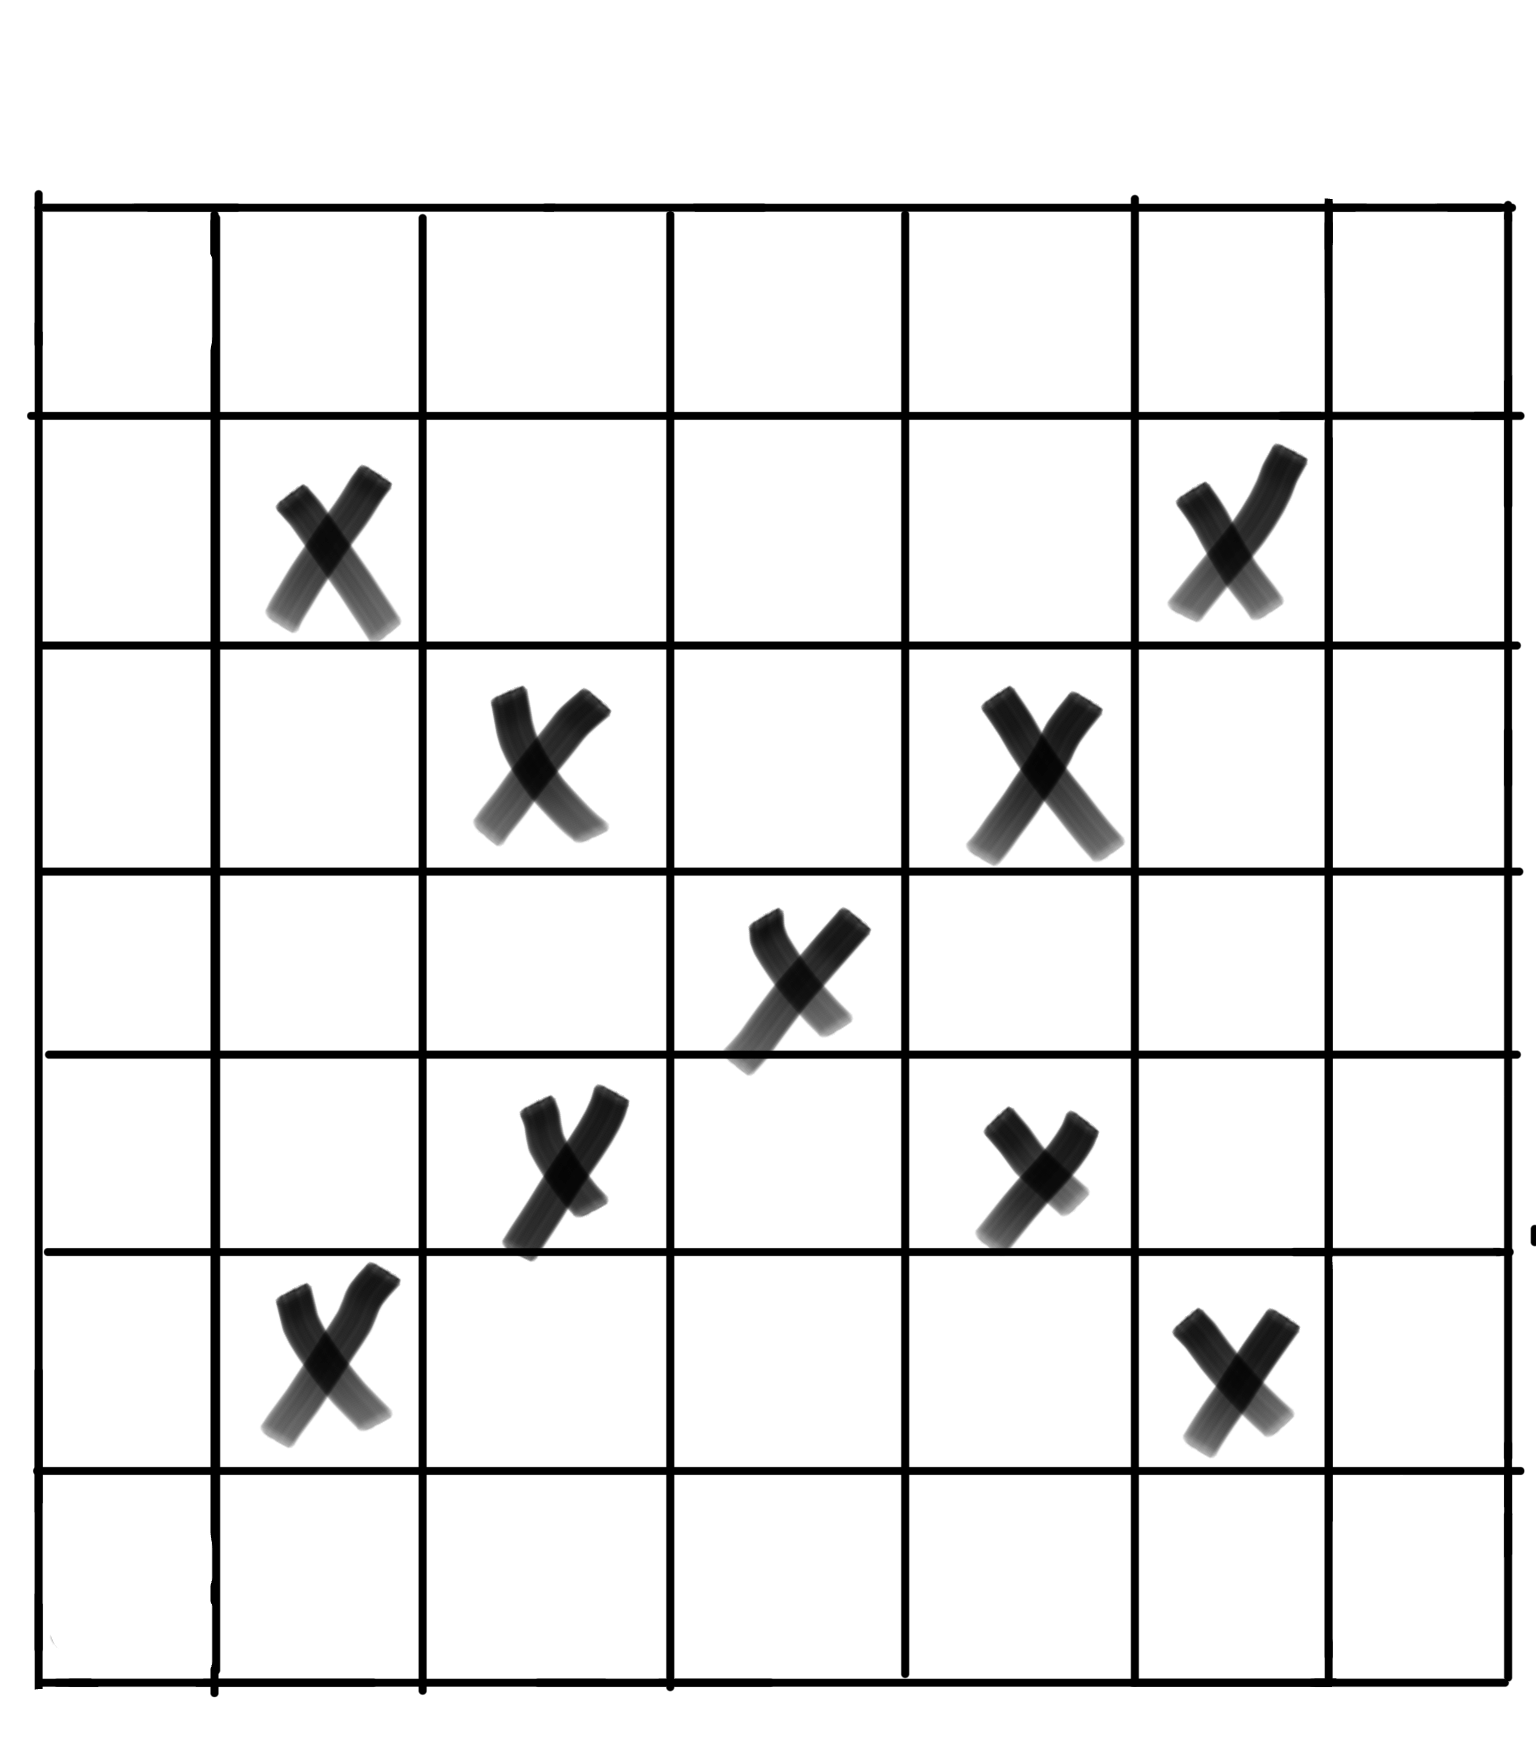
\includegraphics[width=\textwidth]{img/X.png}
    \caption{Letter X in a 7x7 image.}
    \label{fig:x_7x7_image}
  \end{minipage}
  \hfill
  \begin{minipage}[b]{0.4\textwidth}
    \centering
    $\begin{bmatrix}
    0 & 0 & 0 & 0 & 0 & 0 & 0\\
    0 & 1 & 0 & 0 & 0 & 1 & 0\\
    0 & 0 & 1 & 0 & 1 & 0 & 0\\
    0 & 0 & 0 & 1 & 0 & 0 & 0\\
    0 & 0 & 1 & 0 & 1 & 0 & 0\\
    0 & 1 & 0 & 0 & 0 & 1 & 0\\
    0 & 0 & 0 & 0 & 0 & 0 & 0
    \end{bmatrix}$
    \caption{Letter X in a 7x7 matrix.}
    \label{fig:x_7x7_matrix}
  \end{minipage}
\end{figure}


\begin{figure}[!tbp]
  \centering
  \begin{minipage}[b]{0.4\textwidth}
    \centering
    $\begin{bmatrix}
    1 & 0 & 0\\
    0 & 1 & 0\\
    0 & 0 & 1
    \end{bmatrix}$
    \caption{A 3x3 convolution kernel.}
    \label{fig:3x3_convolution_kernel}
  \end{minipage}
  \hfill
  \begin{minipage}[b]{0.4\textwidth}
    \centering
    $\begin{bmatrix}
    2 & 0 & 1 & 0 & 1\\
    0 & 3 & 0 & 1 & 0\\
    1 & 0 & 3 & 0 & 1\\
    0 & 1 & 0 & 3 & 0\\
    1 & 0 & 1 & 0 & 2\\
    \end{bmatrix}$
    \caption{A 5x5 feature map.}
    \label{fig:5x5_feature_map}
  \end{minipage}
\end{figure}



After feeding the program as much as data, the program will be trained to find parameters to determine if it is an `X' or not. If it is a grey-scale picture, each number is not 0 and 1, but a grey-scale value from 0 to 255. If it's a colour image, then it's RGB colours. Essentially, no matter what the image is, the image can end up replacing itself with a bunch of numbers, and that a bunch of numbers can be an input of the training neural network. The goal of training is to find the parameters that make the loss function smallest.\\

But if we use the method described above to train real-world images, it is time-consuming and computationally expensive. Besides, once the image is a little bit deflated and rotated, or changed, then the algorithm will not recognize it. But our eyes are very efficient: if I see a car and a motorcycle once, I can immediately tell the difference between them, and the next time I see the motorcycle, even if the motorcycle has changed direction, position, or is broken, we can still recognize it as a motorcycle and not a car.\\


In 1981, the Nobel Prize in Physiology or Medicine was awarded to two neuroscientists, David Hubel and Wiesel. These two scientists experimented with cats, inserting electrodes into their brains and then showing them a variety of different images to study the results of their brain responses~\cite{hubel1962receptive}. They found that there are two types of cortical fields in the brain related to vision. The first one is called `simple cortical fields', which is characterized by sensitivity to certain lines. After the appearance of lines in a certain direction, these fields will be more sensitive and can see it. There are `complex cortical fields' as well. These complex fields are not only able to respond to lines, but it is also able to respond to the movement of the objects.\\


Later, inspired by them, a Japanese scientist named Kunihiko Fukushima proposed a model called the Neocognitron Model, which explains how a person can see whether the object is a cat or a dog~\cite{fukushima1982neocognitron}. He proposed that there are many layers in the human brain. The visual signals are processed layer by layer. After light enters the eye from the outside, it enters the first layer, then the second layer, then the third layer, and so on. Each layer processes the signal differently. In the beginning, when the light enters the retina, the human eye actually sees a large number of pixels. In the first layer, these pixels abstract some features, such as edges. Then the next layer combines these features to form the outline of the object and more details of the object. Finally, the contours and details are combined into a whole to make a final judgment.\\


Based on this principle, Yann LeCun invented a practical method for image recognition, called convolutional neural network~\cite{lecun1995convolutional}. The role of convolution is to use a mathematical method to extract these features from the image. The way to extract the features is to use a convolution kernel to do the convolution operation. The convolution kernel is also a matrix and is usually a 3x3 or 5x5 matrix. For instance, if we have a convolution kernel which is a 3x3 kernel, and the numbers in it are shown in Figure~\ref{fig:3x3_convolution_kernel}, then a convolution operation will be done with this kernel and the matrix shown in Figure~\ref{fig:x_7x7_matrix}. The operation result is shown in Figure~\ref{fig:5x5_feature_map}. This result is also known as a feature map.\\


In fact, the feature map reinforces the features of the convolution kernel. If you look carefully, you will see that this convolution kernel (Figure~\ref{fig:3x3_convolution_kernel}) only has three oblique blocks of pixels being ones. So if the original matrix (Figure~\ref{fig:x_7x7_matrix}) also has oblique pixel blocks of ones, the number would be extensive when they do the convolution operation. That means we have extracted this feature. The smaller the value of the pixel block in the other positions, the less it satisfies the feature. In a word, with different convolution kernels, we can get different feature maps.\\

The next step after convolution is pooling. This feature map (Figure~\ref{fig:5x5_feature_map}) has a relative large number of elements. For instance, the top left corner has a feature of a line to the bottom right. But the presence of `2' and `3' at the top left of the matrix means that the two zeros around them don't really mean much. So we can simplify it by zooming in on the part of this feature map that has features and ignore the part that doesn't have features. We can use a maximum pooling method. That is, we can extract the largest number from these four numbers (2x2 matrix). Eventually, it can be pooled into a relatively small feature map (Figure~\ref{fig:3x3_feature_map_after_pooling}).\\

\begin{figure}[b]
  \centering
  \begin{minipage}[b]{0.4\textwidth}
    \centering
    $\begin{bmatrix}
    3 & 1 & 1\\
    1 & 3 & 1\\
    1 & 1 & 2
    \end{bmatrix}$
    \caption{A 3x3 feature map after pooling.}
    \label{fig:3x3_feature_map_after_pooling}
  \end{minipage}
  \hfill
  \begin{minipage}[b]{0.4\textwidth}
    \centering
    $\begin{bmatrix}
    0.95 & 0.73 & 0.73\\
    0.73 & 0.95 & 0.73\\
    0.73 & 0.73 & 0.88
    \end{bmatrix}$
    \caption{A 3x3 feature map after activating with sigmoid function.}
    \label{fig:3x3_feature_map_after_activating}
  \end{minipage}
\end{figure}

The step after pooling is activation. The essence of the activation function is to introduce nonlinear factors to solve problems that a linear model cannot solve. Suppose the activation function is a sigmoid function, i.e.,

\begin{equation}
    S(x) =  \frac{\mathrm{1} }{\mathrm{1} + e^{-x} }.
\end{equation}

After activating the sigmoid function, each element in the feature map would be between 0 to 1, as shown in Figure~\ref{fig:3x3_feature_map_after_activating}.\\

It is worth noting that the initial convolution kernel may be artificially set. But later on in the process of machine learning, it will go backwards to adjust and find the most suitable convolution kernel based on its own data, just like the above-mentioned method of using training to adjust the parameters is no different. Since a picture will generally have many features, there will be many corresponding convolution kernels. After many times of convolutions and poolings, features can be found, such as the slanted lines of image, the contours, and the colour features. We take this enough information and then feed it into this fully connected network for training, and finally, we can determine what this image really is.\\

In Sec~\ref{sec2.2}, recent literature and development of Convolutional Neural Networks were discussed. However, a number of convolutional neural network-based object detection frameworks have recently emerged that can run faster, have a higher detection accuracy, have cleaner results and are easier to develop. Contrastingly, compared to the Faster RCNN model, the YOLO model can better detect smaller objects, for example by easily detecting smaller traffic lights at a distance~\cite{Dwivedi2020YOLOv5} (Figure~\ref{fig:who_wins_traffic_light_YOLO}, Figure~\ref{fig:who_wins_traffic_light_RCNN}), which is important when detecting satellite images. Also, the YOLO model has a faster end-to-end runtime and detection accuracy than the Faster RCNN. The figures below is from a YouTube clip of an NBA game. As seen in Figure~\ref{fig:who_wins_nba_YOLO} and Figure~\ref{fig:who_wins_nba_RCNN}, the detection accuracy under the YOLO model is more accurate than that of the Faster RCNN. This helps to monitor the number of small boats in real time using the YOLO model in the future.\\

\begin{figure}[p]
    \centering
    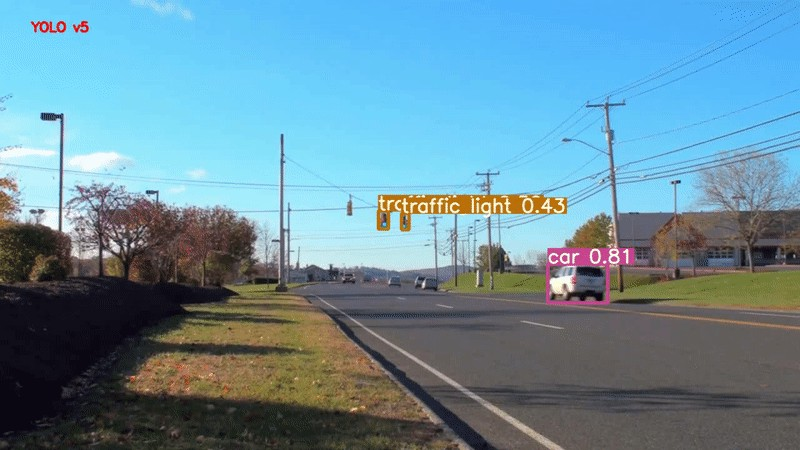
\includegraphics[scale=0.5]{img/who_wins_traffic_light_YOLO.jpg}
    \longcaption{YOLOv5 model in a driving video.}{YOLOv5 model in a driving video~\cite{Dwivedi2020YOLOv5}.}
    \label{fig:who_wins_traffic_light_YOLO}
\end{figure}

\begin{figure}[p]
    \centering
    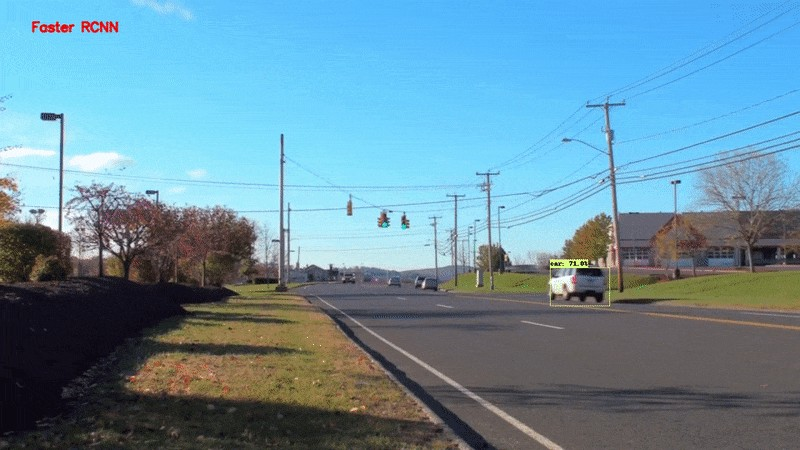
\includegraphics[scale=0.5]{img/who_wins_traffic_light_RCNN.jpg}
    \longcaption{Faster RCNN model in a driving video.}{Faster RCNN model in a driving video~\cite{Dwivedi2020YOLOv5}.}
    \label{fig:who_wins_traffic_light_RCNN}
\end{figure}

\begin{figure}[p]
    \centering
    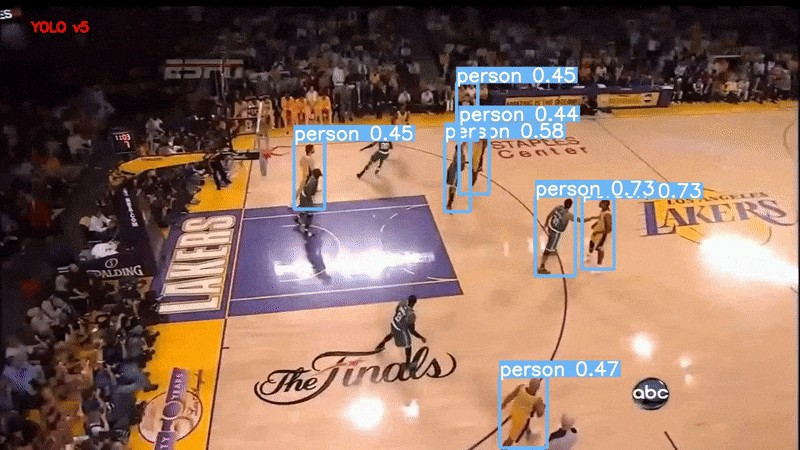
\includegraphics[scale=0.5]{img/who_wins_nba_YOLO.jpg}
    \longcaption{YOLOv5 model in an NBA game video.}{YOLOv5 model in an NBA game video~\cite{Dwivedi2020YOLOv5}.}
    \label{fig:who_wins_nba_YOLO}
\end{figure}

\begin{figure}[p]
    \centering
    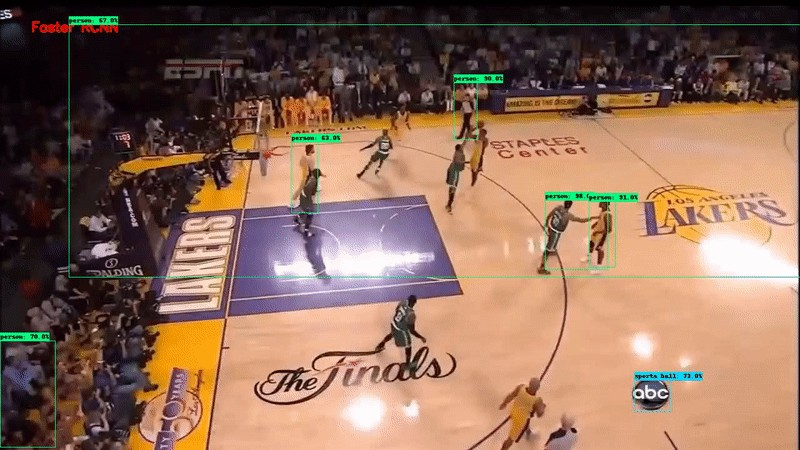
\includegraphics[scale=0.5]{img/who_wins_nba_RCNN.jpg}
    \longcaption{Faster RCNN model in an NBA game video.}{Faster RCNN model in an NBA game video~\cite{Dwivedi2020YOLOv5}.}
    \label{fig:who_wins_nba_RCNN}
\end{figure}


According to the official YOLOv5 tutorial, YOLOv5 has four different categories of models, YOLOv5s, YOLOv5m, YOLOv5l, and YOLOv5x. They have 7.3 million, 21.4 million, 47 million and 87.7 million parameters respectively. The official performance charts are also available, as shown in the Figure~\ref{fig:YOLOv5_Performance}.\\

\begin{figure}[h]
    \centering
    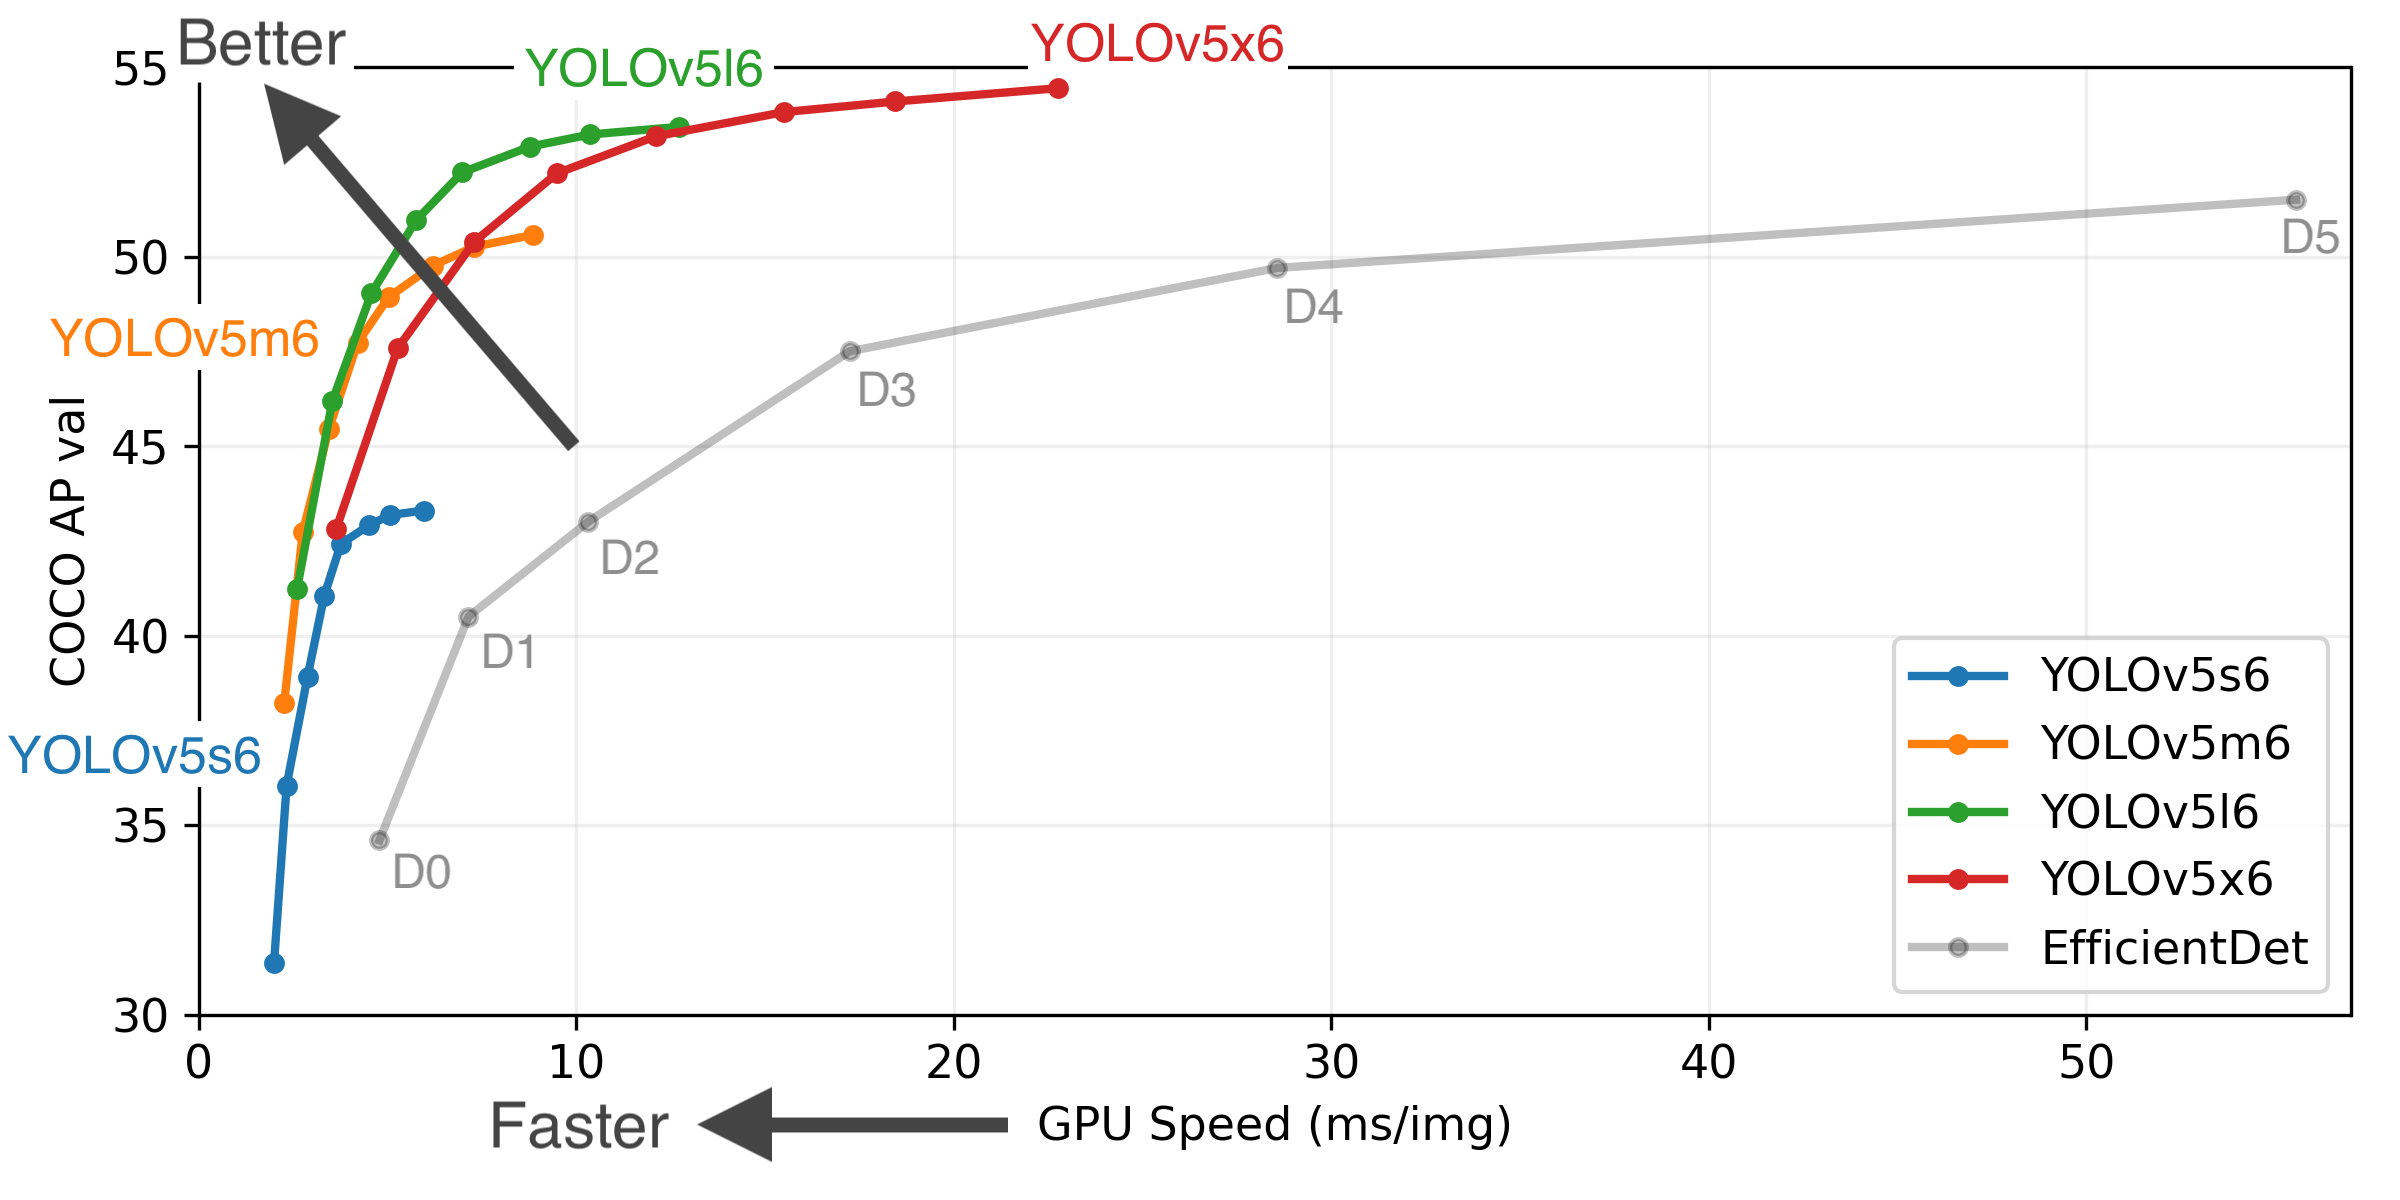
\includegraphics[scale=0.7]{img/YOLOv5_Performance.png}
    \longcaption{COCO Average Precision (AP) vs. GPU Speed in YOLOv5.}{COCO Average Precision (AP) vs. GPU Speed in YOLOv5~\cite{glenn_jocher_2020_4154370}.}
    \label{fig:YOLOv5_Performance}
\end{figure}

Thus, the YOLOv5l model is able to achieve higher average precision with the same faster computing speed. Thus, in this thesis, the YOLOv5l model was chosen as the model for the training dataset.\\



\newpage
\subsection{Data Source and Improvements}
Artificial intelligence algorithms need to be complemented by a large amount of data. An open-source data from a former TU Berlin researcher Tom Lutherborrow at Kaggle was used in this thesis. This open-source data contains 794 high-resolution images of ships from Google Earth~\cite{lutherborrowship}. However, this dataset is too much large than expected. Each image is larger than 9 megabytes, which is an efficiency burden for the training of neural networks, especially when there are few objects to be detected. With the tool RoboFlow, each training image can be resized to a 416x416 pixel image.\\


\subsection{Computing Power: CPU or GPU}
Another important foundation of artificial intelligence is computing power. For example, in this convolutional neural network algorithm that we have just done, each calculation is actually not very complicated: it is just addition and multiplication. But the amount of computation is huge. For instance, there is an image that is 800x600, but due to the RGB colours, there are around 1.44 million pixels in total. Using a 3x3x3 convolution kernel will take about 13 million multiplications and about 12 million additions. It's simple addition and multiplication, but it's a vast number of operations. Besides, that's just using a convolution kernel for a simple image. There are actually thousands of images convolved thousands of times during the training process, so that's a vast number of operations.\\

The GPU was originally meant to be a graphics processing unit, and it has a parallel structure that allows for more efficient computing than a central processing unit (CPU). For instance, if a link in a neural network is being computed simultaneously with another link, a large number of small cores can be used simultaneously to speed up the computation. In this thesis, all ConvNet models were trained using a YOLOv5 framework with Tesla P100 GPU in the Google Colab.\\




\section{Algorithms for Detection and Classification}
\subsection{Target Areas in the Gulf of California}
\label{sec3.2.1}
The Gulf of Californian was chosen as an area of study for this thesis. Ideally, in order to analyse a sufficient amount of satellite image data, the ports of each of the major harbour cities in the Gulf of California would need to be included in the scope of our study. Thus, it was worth to finding out if there was enough data for the area in Google Earth Pro. The results of the statistics can be seen in Table~\ref{table:baja_california_dates}, Table~\ref{table:Baja_California_Sur_dates}, Table~\ref{table:Sonora_dates}, Table~\ref{table:Sinaloa_dates}, Table~\ref{table:Nayarit_dates}, Table~\ref{table:Jalisco_dates}, Table~\ref{table:Colima_dates}.\\

In fact, Google Earth Pro provided very little image data than was expected. Most of the Mexican cities in the Gulf of California do not have satellite data for 2021. A few cities have satellite data from 2018. More cities have satellite data for 2019 and 2020. This reflects that:
\begin{itemize}
    \item a steady increase in the collection of satellite data in the Gulf of California.
    \item that the free, high-quality satellite data available from Google Earth Pro is not immediately available for publication.
    \item regional differences in satellite data are still evident. Some cities, such as Guaymas, will have access to about 15 satellite images a year in 2019 or 2020. However, some cities, such as La Ventana, did not appear in Google Earth Pro in 2019 and 2020, when almost all other cities have been photographed by satellite.\\
\end{itemize}

For this reason, it is clear that continuing with the previous strategy of analysing the satellite data for each city in the Gulf of California (from Table~\ref{table:baja_california_dates} to Table~\ref{table:Jalisco_dates}) would lead to a relatively large information bias and thus would not achieve an accurate result of the composition of the boats of the Gulf of California. Therefore, the following three cities with the most data in Google Earth Pro were finally chosen as the target areas for this thesis: Santa Rosalia, Loreto, Guaymas.\\

% Table 3.1
\begin{table}[h!]
\centering
\begin{tabular}{ l | p{2.5cm} | p{2.5cm} | p{2.5cm} | p{2.5cm} }
\toprule
City & 2021 & 2020 & 2019 & 2018 \\
\midrule
San Felipe & NA & 12/30; 12/26; 12/9; 11/17; 11/1; 4/19 & 6/17; 2/5; 1/22 & 10/23; 9/29; 3/3; 3/1; 2/26; 2/5\\
\midrule
Bahia de los Angeles & NA & 5/15 & 6/17 & 11/10\\
\midrule
Isla Smith & NA & NA & 6/17 & NA\\
\bottomrule
\end{tabular}
\caption{Specific dates when Google Earth Pro has images from 2018 to 2021 in Baja California, Meico.}
\label{table:baja_california_dates}
\end{table}


% Table 3.4
\begin{table}[h!]
\centering
\begin{tabular}{ l | p{2.5cm} | p{2.5cm} | p{2.5cm} | p{2.5cm} }
\toprule
City & 2021 & 2020 & 2019 & 2018 \\
\midrule
Los Mochis & 2/1; 1/31 & 12/2; 9/30; 9/15; 9/12; 4/20; 1/29; 1/18 & 12/8; 8/3; 7/12; 6/13; 4/30; 2/7 & 11/6; 10/20; 7/3\\
\midrule
La Cruz & 1/16 & 10/31; 2/25; 2/21 & 10/29; 8/1; 7/10; 6/20; 4/19; 1/27 & 11/3; 10/16; 8/9; 1/17\\
\midrule
Mazatlan & NA & 10/31; 10/1; 9/19; 9/10; 8/29; 7/21; 2/28; 1/26; 1/18 & 12/7; 11/30; 8/3 & 11/3; 10/30; 10/27; 10/24; 10/12; 8/4; 6/27; 5/11; 4/19; 1/12\\
\bottomrule
\end{tabular}
\caption{Specific dates when Google Earth Pro has images from 2018 to 2021 in Sinaloa, Meico.}
\label{table:Sinaloa_dates}
\end{table}

% Table 3.7
\begin{table}[h!]
\centering
\begin{tabular}{ l | p{2.5cm} | p{2.5cm} | p{2.5cm} | p{2.5cm} }
\toprule
City & 2021 & 2020 & 2019 & 2018 \\
\midrule
Manzanillo & NA & 12/26; 9/14; 5/31; 3/3; 1/12 & 12/9; 3/7; 3/6 & NA\\
\bottomrule
\end{tabular}
\caption{Specific dates when Google Earth Pro has images from 2018 to 2021 in Colima, Meico.}
\label{table:Colima_dates}
\end{table}


% Table 3.2
\begin{table}[p]
\centering
\begin{tabular}{ l | p{2.5cm} | p{2.5cm} | p{2.5cm} | p{2.5cm} }
\toprule
City & 2021 & 2020 & 2019 & 2018 \\
\midrule
Santa Rosalia & NA & 12/21; 12/9; 11/28; 11/1; 9/11; 8/11; 8/6; 7/17; 7/14; 7/10; 7/6; 6/22; 6/17; 6/9; 5/26; 5/18; 5/8; 4/26; 4/18; 4/14; 3/15; 2/14; 2/3; 1/28; 1/27; 1/22; 1/13; 1/5 & 12/19; 12/14; 12/11; 12/3; 10/31; 10/20; 9/24; 9/20; 9/9; 8/26; 8/21; 8/11; 7/8; 7/5; 4/17; 1/30 & 11/9; 7/4; 6/7; 4/2; 2/23\\
\midrule
Mulege & 1/18 & NA & 7/8 & NA\\
\midrule
Loreto & 2/12; 1/18 & 11/25; 11/23; 11/22; 11/4; 9/26; 9.13; 8/25; 8/17; 8/14; 7/29; 7/25; 7/16; 7/14; 7/10; 6/25; 6/3; 4/30; 4/23; 4/22; 4/18; 4/11; 3/16; 2/25; 1/29; 1/18; 1/2 & 12/30; 12/11; 11/1; 10/31; 10/7; 10/4; 9/26; 8/27; 8/26; 8/19; 7/9; 6/22; 4/26; 4/11; 1/30 & 10/2; 9/26; 8/14\\
\midrule
La Paz & NA & 1/18 & NA & 4/4\\
\midrule
La Ventana & NA & NA & NA & 4/4\\
\midrule
San Jose del Cabo & NA & NA & NA & 3/28\\
\midrule
Cabo San Lucas & NA & 3/28 & NA & 3/28\\
\bottomrule
\end{tabular}
\caption{Specific dates when Google Earth Pro has images from 2018 to 2021 in Baja California Sur, Meico.}
\label{table:Baja_California_Sur_dates}
\end{table}


% Table 3.3
\begin{table}[p]
\centering
\begin{tabular}{ l | p{2.5cm} | p{2.5cm} | p{2.5cm} | p{2.5cm} }
\toprule
City & 2021 & 2020 & 2019 & 2018 \\
\midrule
Golfo de Santa Clara & 1/9 & NA & 6/24 & NA\\
\midrule
Puerto Penasco & 1/26 & 8/27; 8/19; 7/28; 2/15 & 11/30; 11/7; 10/15; 10/12; 10/1; 6/19; 6/17; 2/15; 2/12; 2/7; 1/27; 1/25 & 10/10; 9/29; 9/13\\
\midrule
Bahia de Kino & 1/10 & NA & 6/25; 6/18 & NA\\
\midrule
Guaymas & 2/10 & 12/9; 11/28; 11/9; 10/24; 9/24; 8/23; 8/17; 8/9; 7/26; 7/10; 5/27; 5/13; 4/23; 4/14; 3/6; 2/6; 2/1; 1/29; 1/7 & 11/13; 11/1; 9/15; 7/15; 6/21; 6/20; 6/13; 6/9; 4/24; 4/19; 3/9; 2/4; 1/19 & 11/1; 7/20; 3/16; 1/22\\
\bottomrule
\end{tabular}
\caption{Specific dates when Google Earth Pro has images from 2018 to 2021 in Sonora, Meico.}
\label{table:Sonora_dates}
\end{table}


% Table 3.5
\begin{table}[p]
\centering
\begin{tabular}{ l | p{2.5cm} | p{2.5cm} | p{2.5cm} | p{2.5cm} }
\toprule
City & 2021 & 2020 & 2019 & 2018 \\
\midrule
San Blas & NA & 1/6 & 2/27 & 10/11; 5/7; 4/10; 2/27\\
\bottomrule
\end{tabular}
\caption{Specific dates when Google Earth Pro has images from 2018 to 2021 in Nayarit, Meico.}
\label{table:Nayarit_dates}
\end{table}


% Table 3.6
\begin{table}[p]
\centering
\begin{tabular}{ l | p{2.5cm} | p{2.5cm} | p{2.5cm} | p{2.5cm} }
\toprule
City & 2021 & 2020 & 2019 & 2018 \\
\midrule
Puerto Vallarta & NA & 5/1; 3/28 & NA & 3/27; 3/21; 3/19\\
\bottomrule
\end{tabular}
\caption{Specific dates when Google Earth Pro has images from 2018 to 2021 in Jalisco, Meico.}
\label{table:Jalisco_dates}
\end{table}



\subsection{Image Kernel and Image Sharpening}
\label{sec3.2.2}
Similar to the principle of using convolution kernels, specific image kernels can sharpen the image. While the sharpening kernel does not make the image higher resolution, it emphasises the differences in adjacent pixel values which makes the image look more vivid. Overall, with the same model weight, as shown in Figure~\ref{fig:sharpening}, sharpening an image can significantly improve the recognition accuracy of an image with a 5x5 image kernel.\\

\begin{figure}[h!]
\centering
\begin{subfigure}[p]{0.7\textwidth}
    \centering
    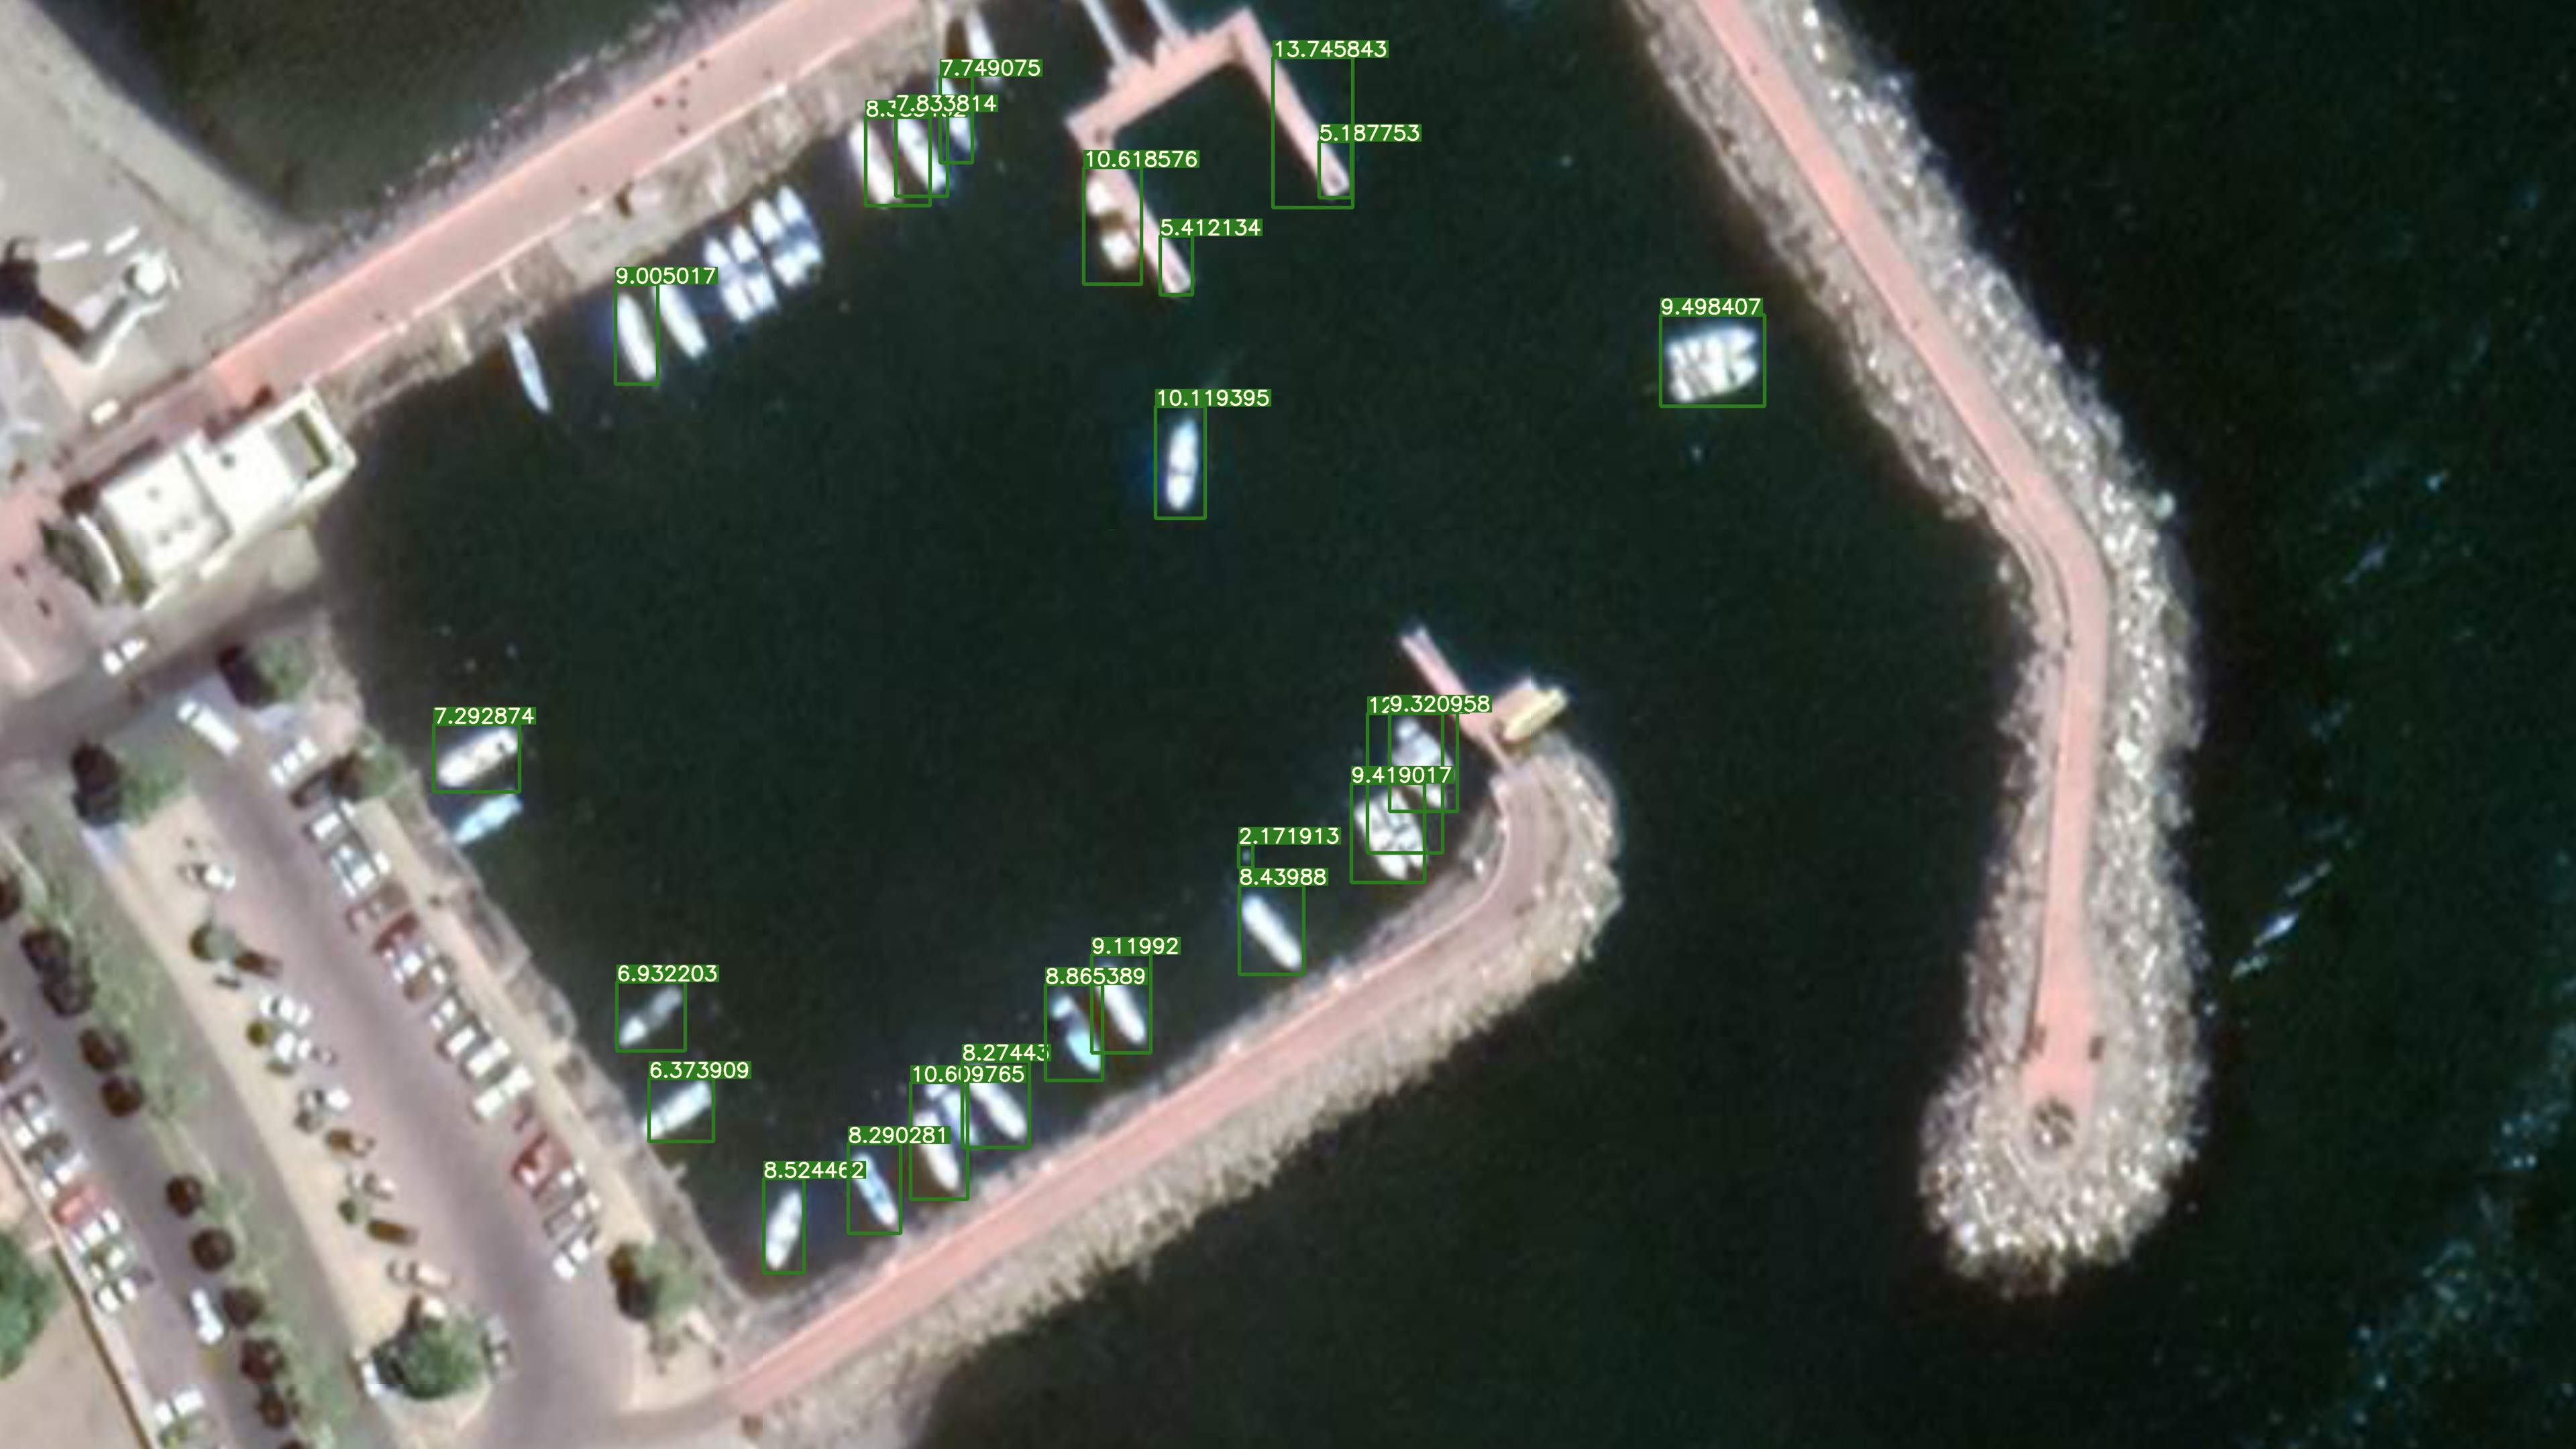
\includegraphics[width=1\linewidth]{img/before_sharpening.jpg}
    \caption{Detection before sharpening.}
    \label{fig:before_sharpening}
\end{subfigure}

\begin{subfigure}[p]{0.7\textwidth}
    \centering
    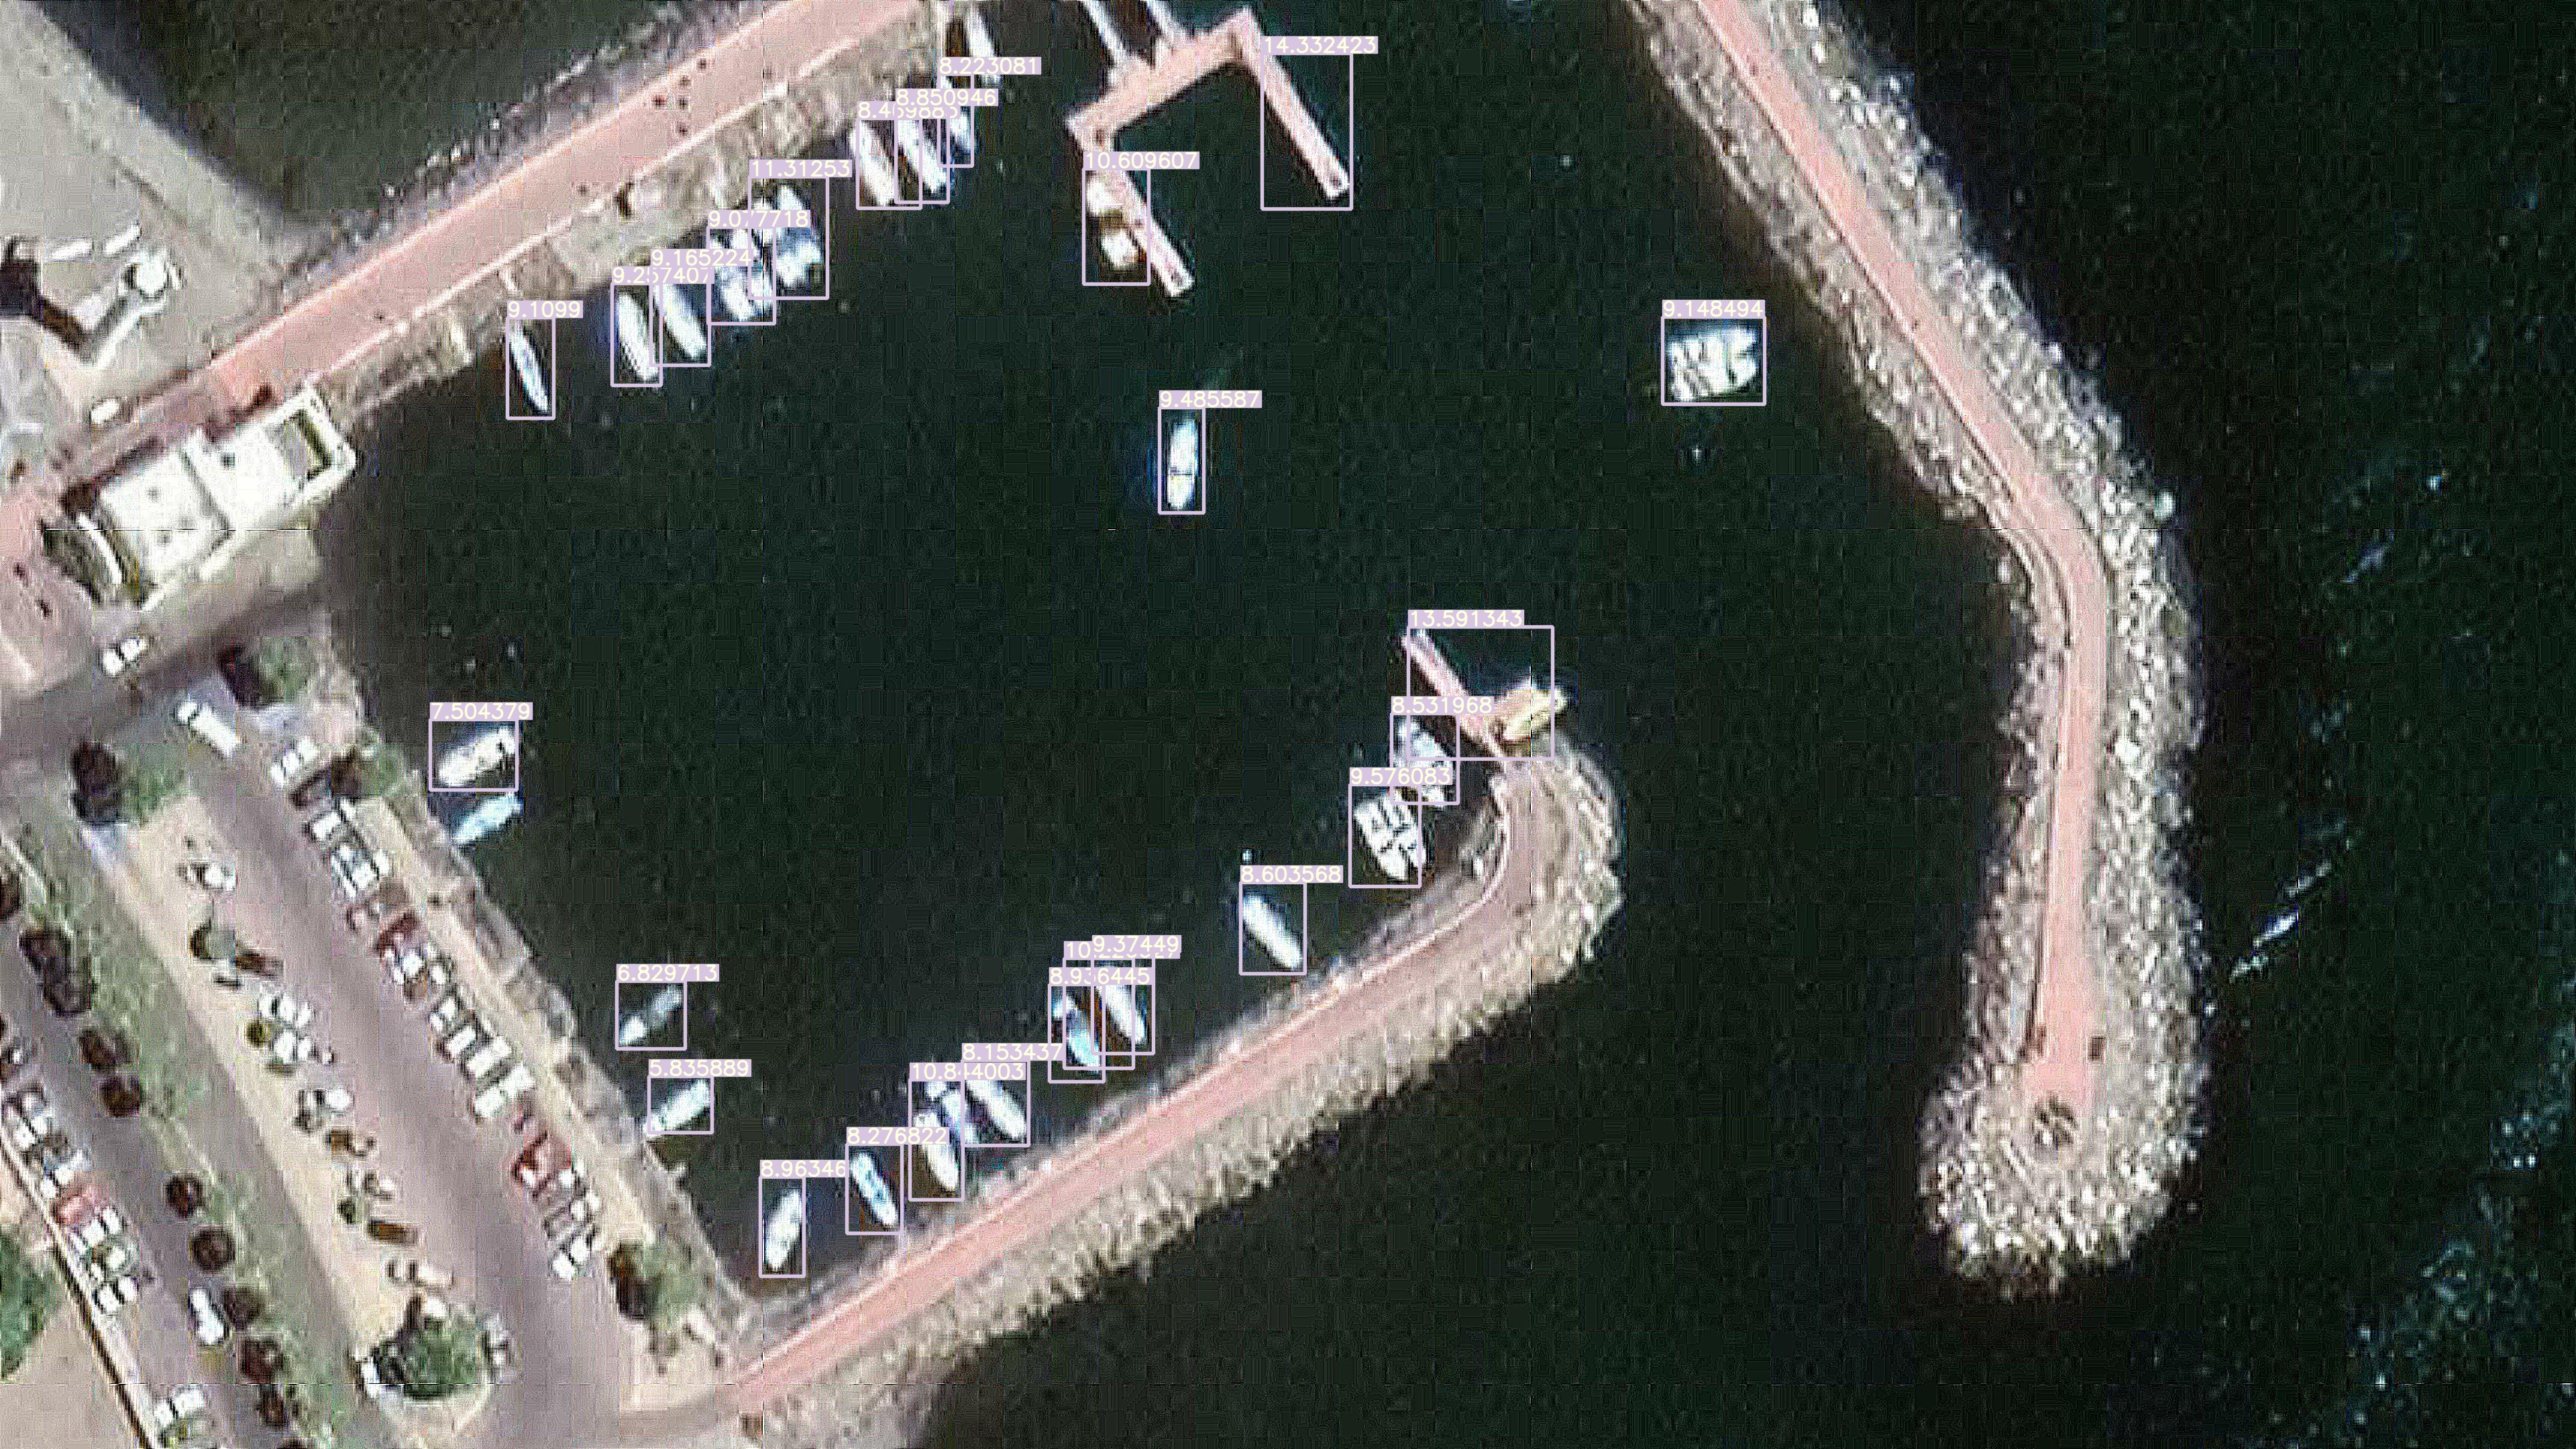
\includegraphics[width=1\linewidth]{img/after_sharpening.jpg}
    \caption{Detection after sharpening.}
    \label{fig:after_sharpening}
\end{subfigure}
\caption{Detections before and after sharpening}
\label{fig:sharpening}
\end{figure}


\newpage
\subsection{Detecting the Length of Small boats}
\label{sec3.2.3}
Measuring the length of a ship is one of the most difficult topics in this thesis. As Google Earth Pro does not provide an application programming interface (API) for accurate scales, manually measuring the size of a particular scale became the core of measuring the size of a ship.\\

As the dataset for the training model was created with each edge tangent to the edge of the detected object, we can roughly treat the boat's length as the length of the diagonal of the detection box. Secondly, since the scale is central to the production of the bay dataset that follows, i.e., the satellite image at this scale:
\begin{itemize}
    \item cannot be too large: they need to contain the full complement of small boats (if any), and the complexity of producing the dataset must also be considered.
    \item cannot be too small: otherwise, there is a tendency for multiple small boats docked together to be detected as a whole party.
    \item be sufficiently clear: the model needs to be allowed to accurately identify the length of small boats to reduce errors in scale.
\end{itemize}

Based on the above rules, the eye altitude was finally determined to be 200m. Meanwhile, I used a satellite image of Zurich Lake, Switzerland, on 16 August 2018 as the standard image for defining the scale (Figure~\ref{fig:zurich}). \\

After metering, the vessel in Figure~\ref{fig:zurich} with a YOLO length of 0.434517 is actually 55.17m. Then, with an eye altitude of 200 metres, the ratio of the real length to the YOLO length is approximately 127. Finally, after several verifications, this ratio is within the margin of error and can be used as a scaling ratio. And having the same ratio and the same eye altitude is not enough. We also need to keep the resolution of each image the same as well. For this purpose, all datasets involved in the detection will maintain a resolution of 3840x2160.\\

\begin{figure}
    \centering
    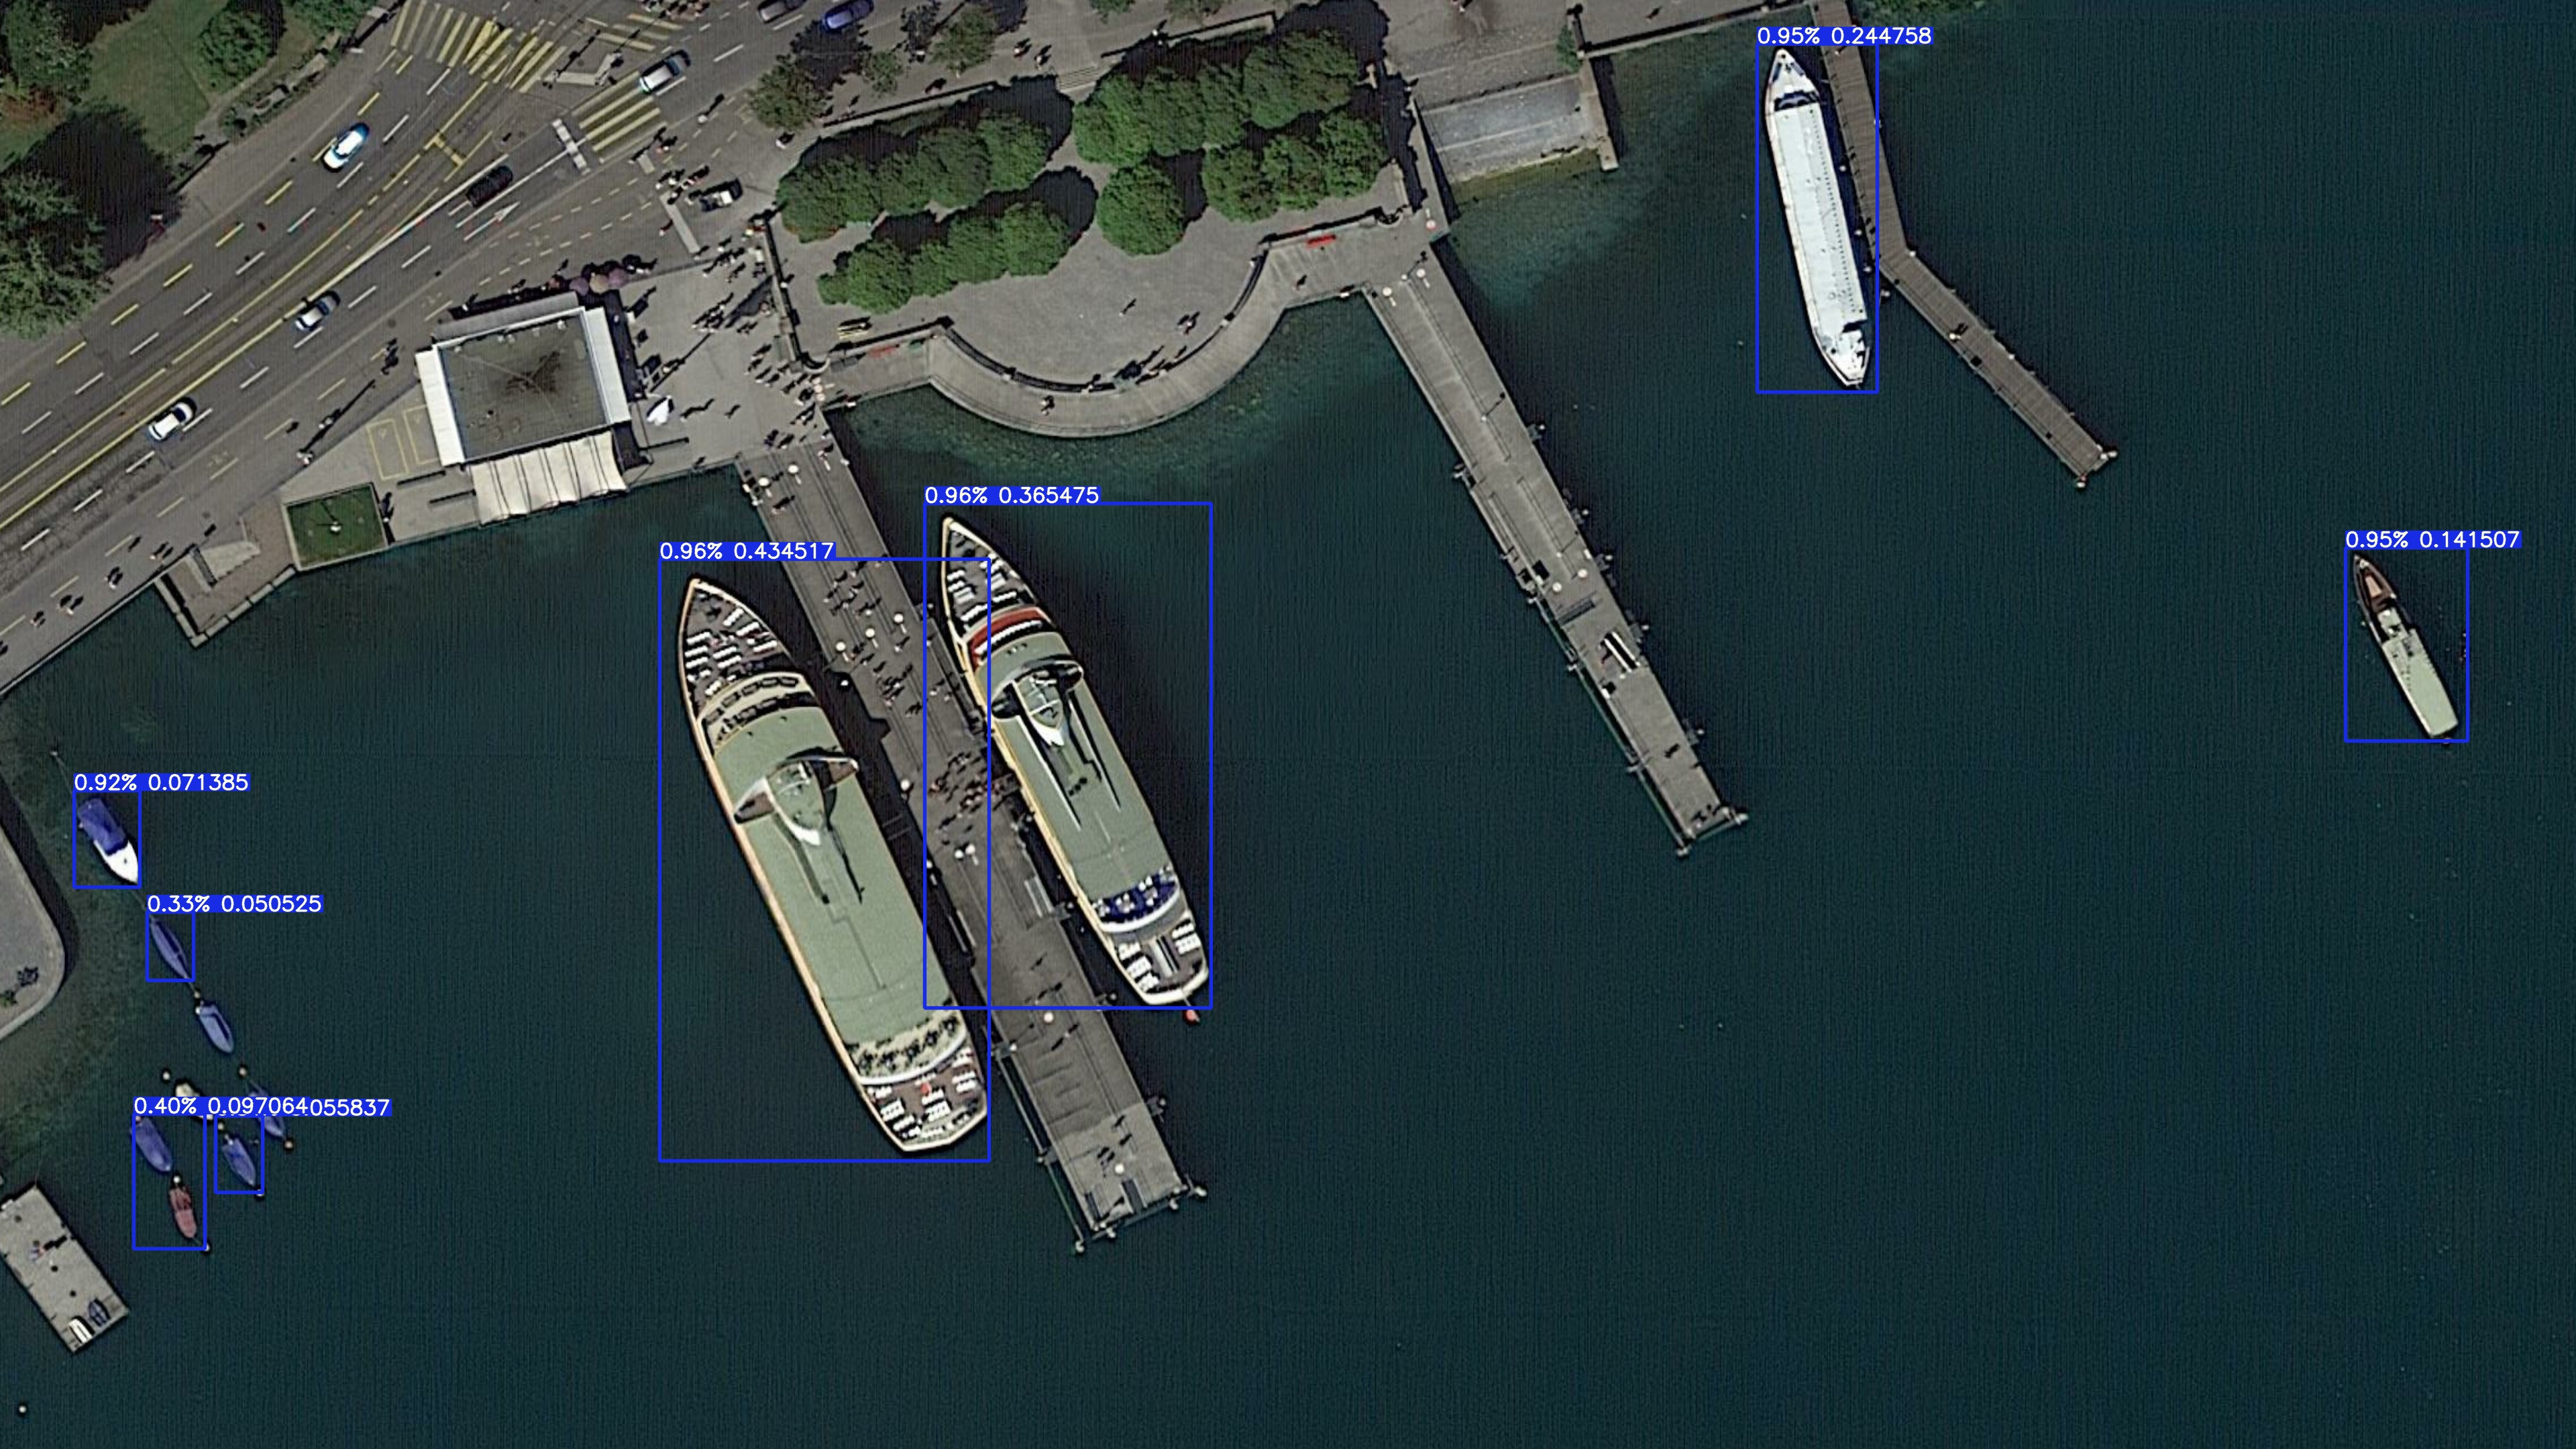
\includegraphics[scale=0.1]{img/zurich.jpg}
    \caption{An image from Google Earth Pro for Zurich Lake on 16 Aug 2018 when eye alt is 200 meters.}
    \label{fig:zurich}
\end{figure}


\newpage
\subsection{Classification of Small Boats and Big Boats}
In a certain sense, large vessels (e.g. cargo ships or warships) and small vessels (e.g. small boats for domestic use for recreation and fishing) are distinguished when creating the dataset for the area. However, due to the scaling, the eye altitude of the image is only 200 meters. Therefore, some enormous vessels, such as cargo ships, do not even appear fully in an image with a resolution of 3840x2160 (such as Figure~\ref{fig:Guaymas_202103_overflow_screen}), i.e., they do not appear in the statistical results. On the other hand, some of the larger vessels, slightly shorter in length, are identified correctly by the algorithm and counted as part of the number of large vessels in the area (Figure~\ref{fig:Guaymas_202105_detect_small_large}).

\begin{figure}
    \centering
    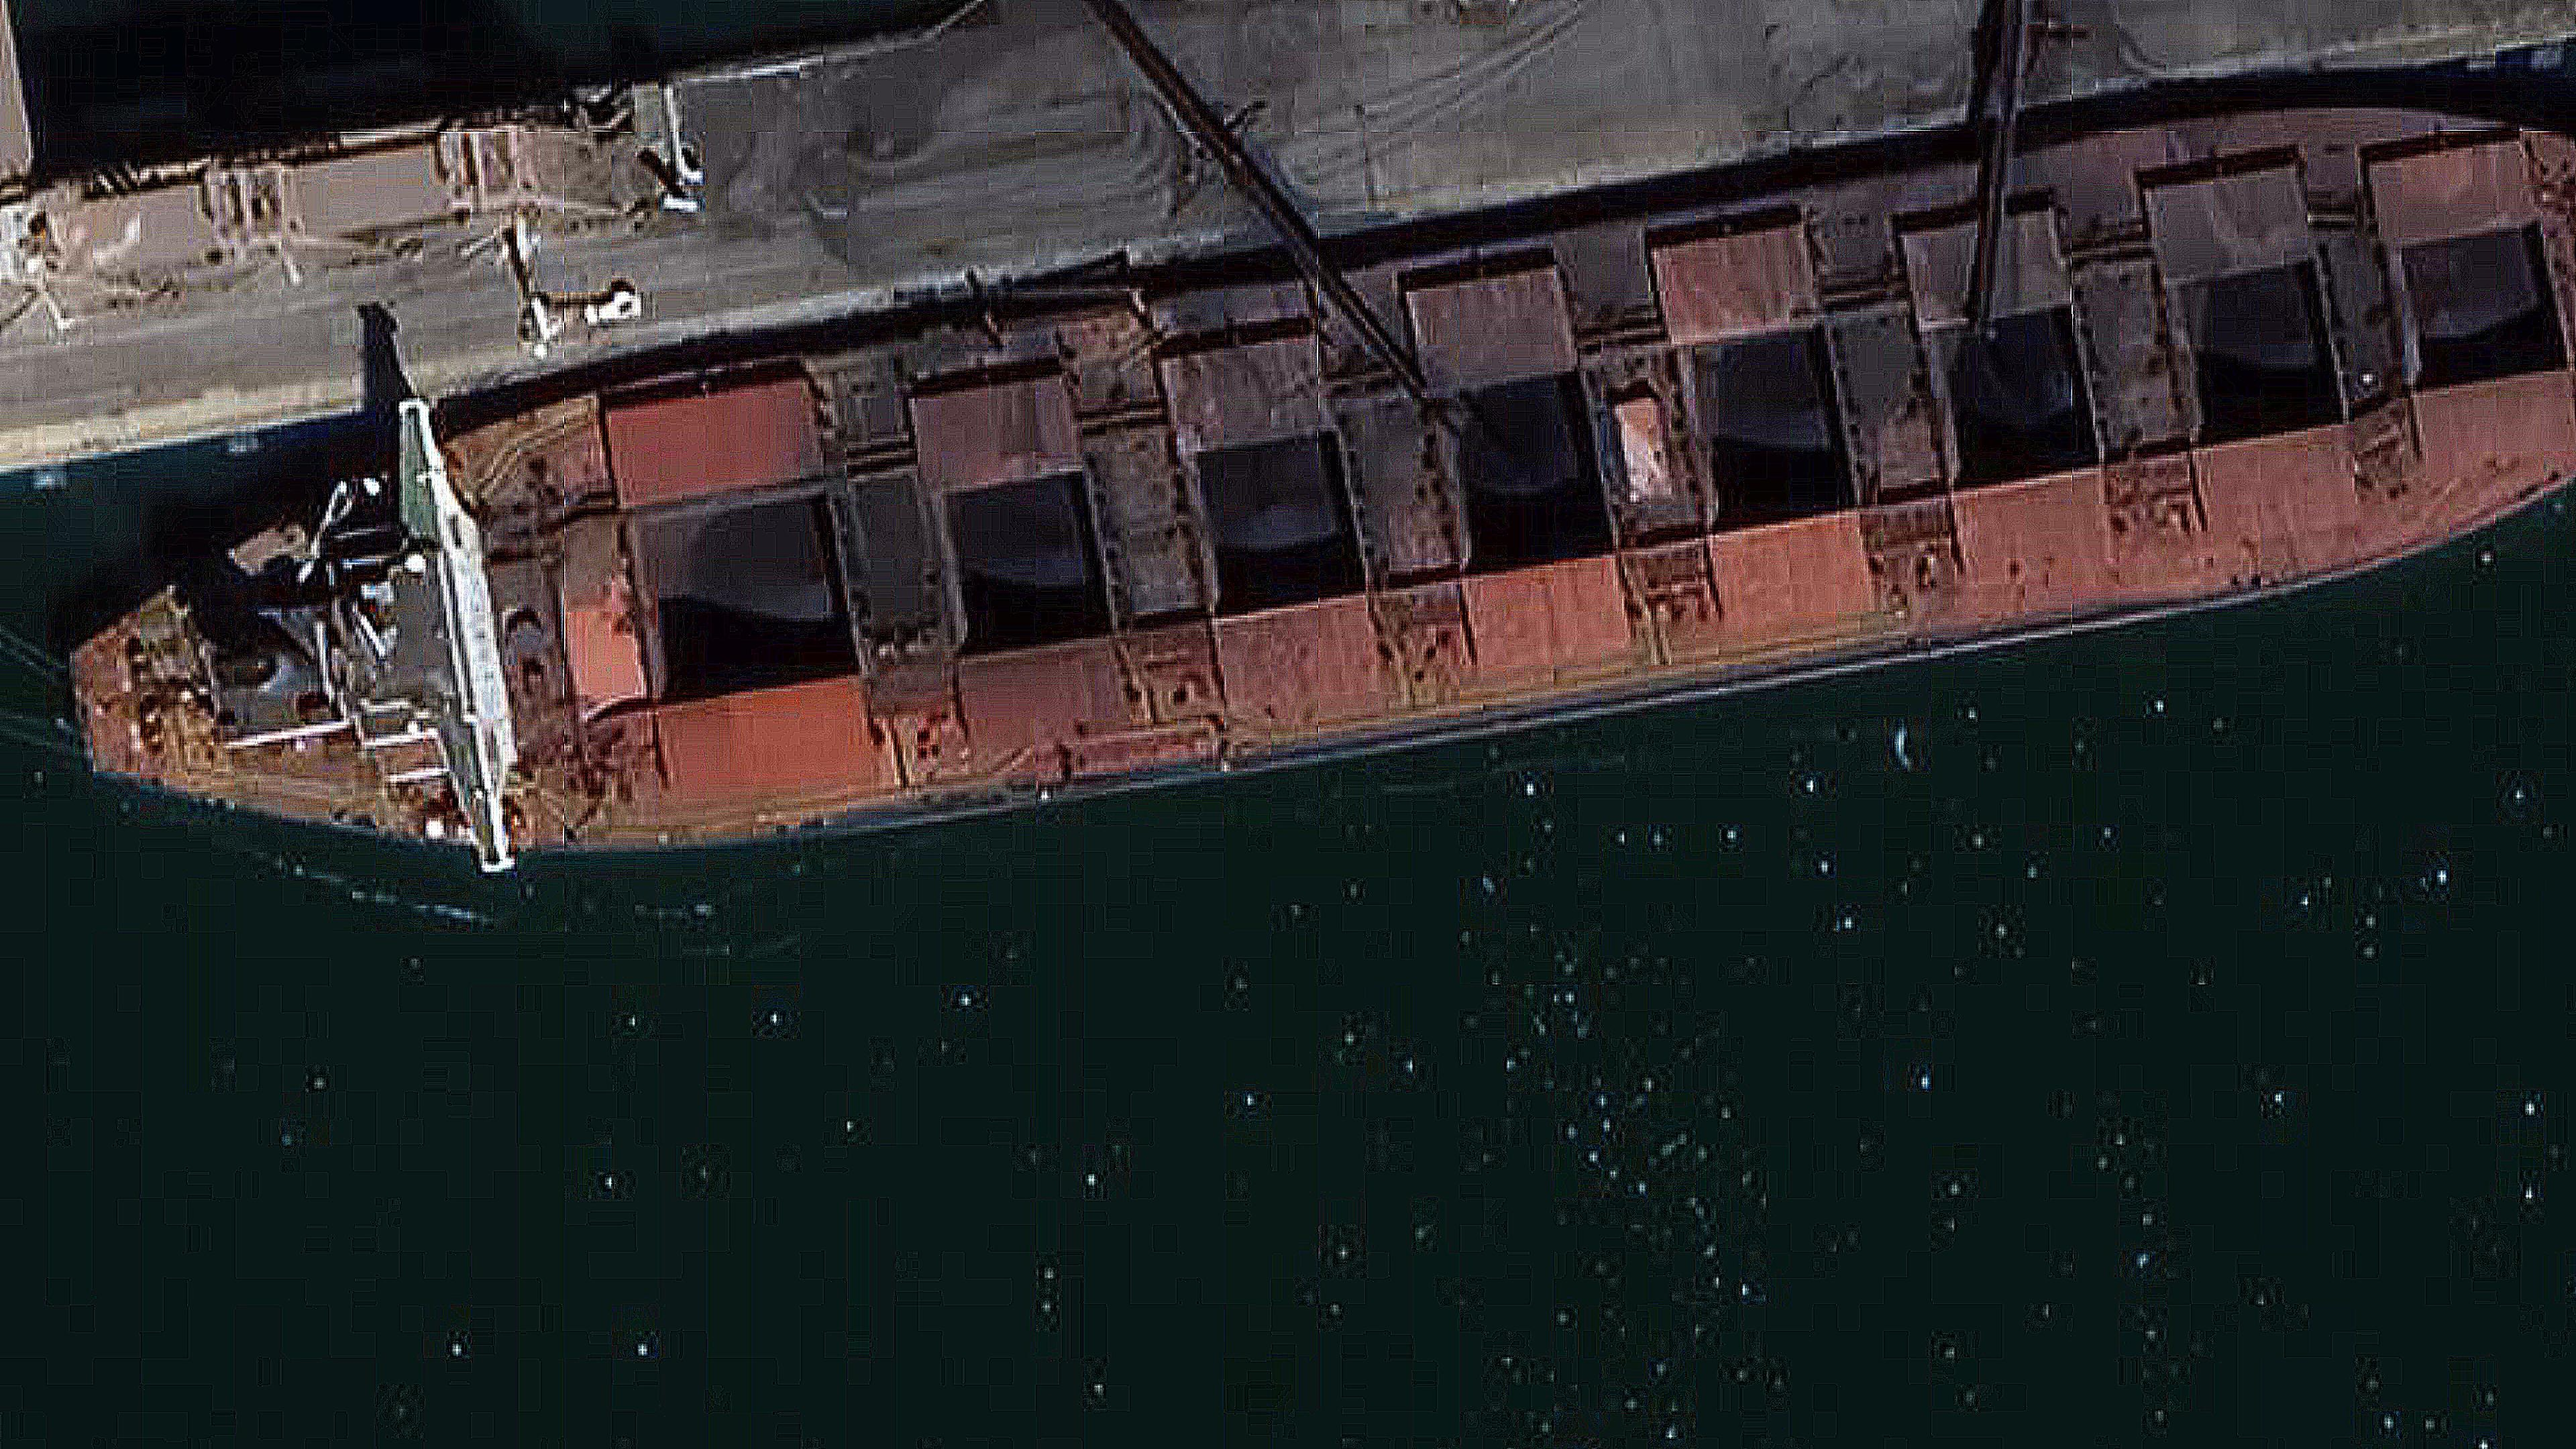
\includegraphics[scale=0.11]{img/Guaymas_202103_overflow_screen.jpg}
    \caption{A cargo (March 2021, Guaymas) overflowed the image and will be excluded from the statistics.}
    \label{fig:Guaymas_202103_overflow_screen}
\end{figure}


\begin{figure}
    \centering
    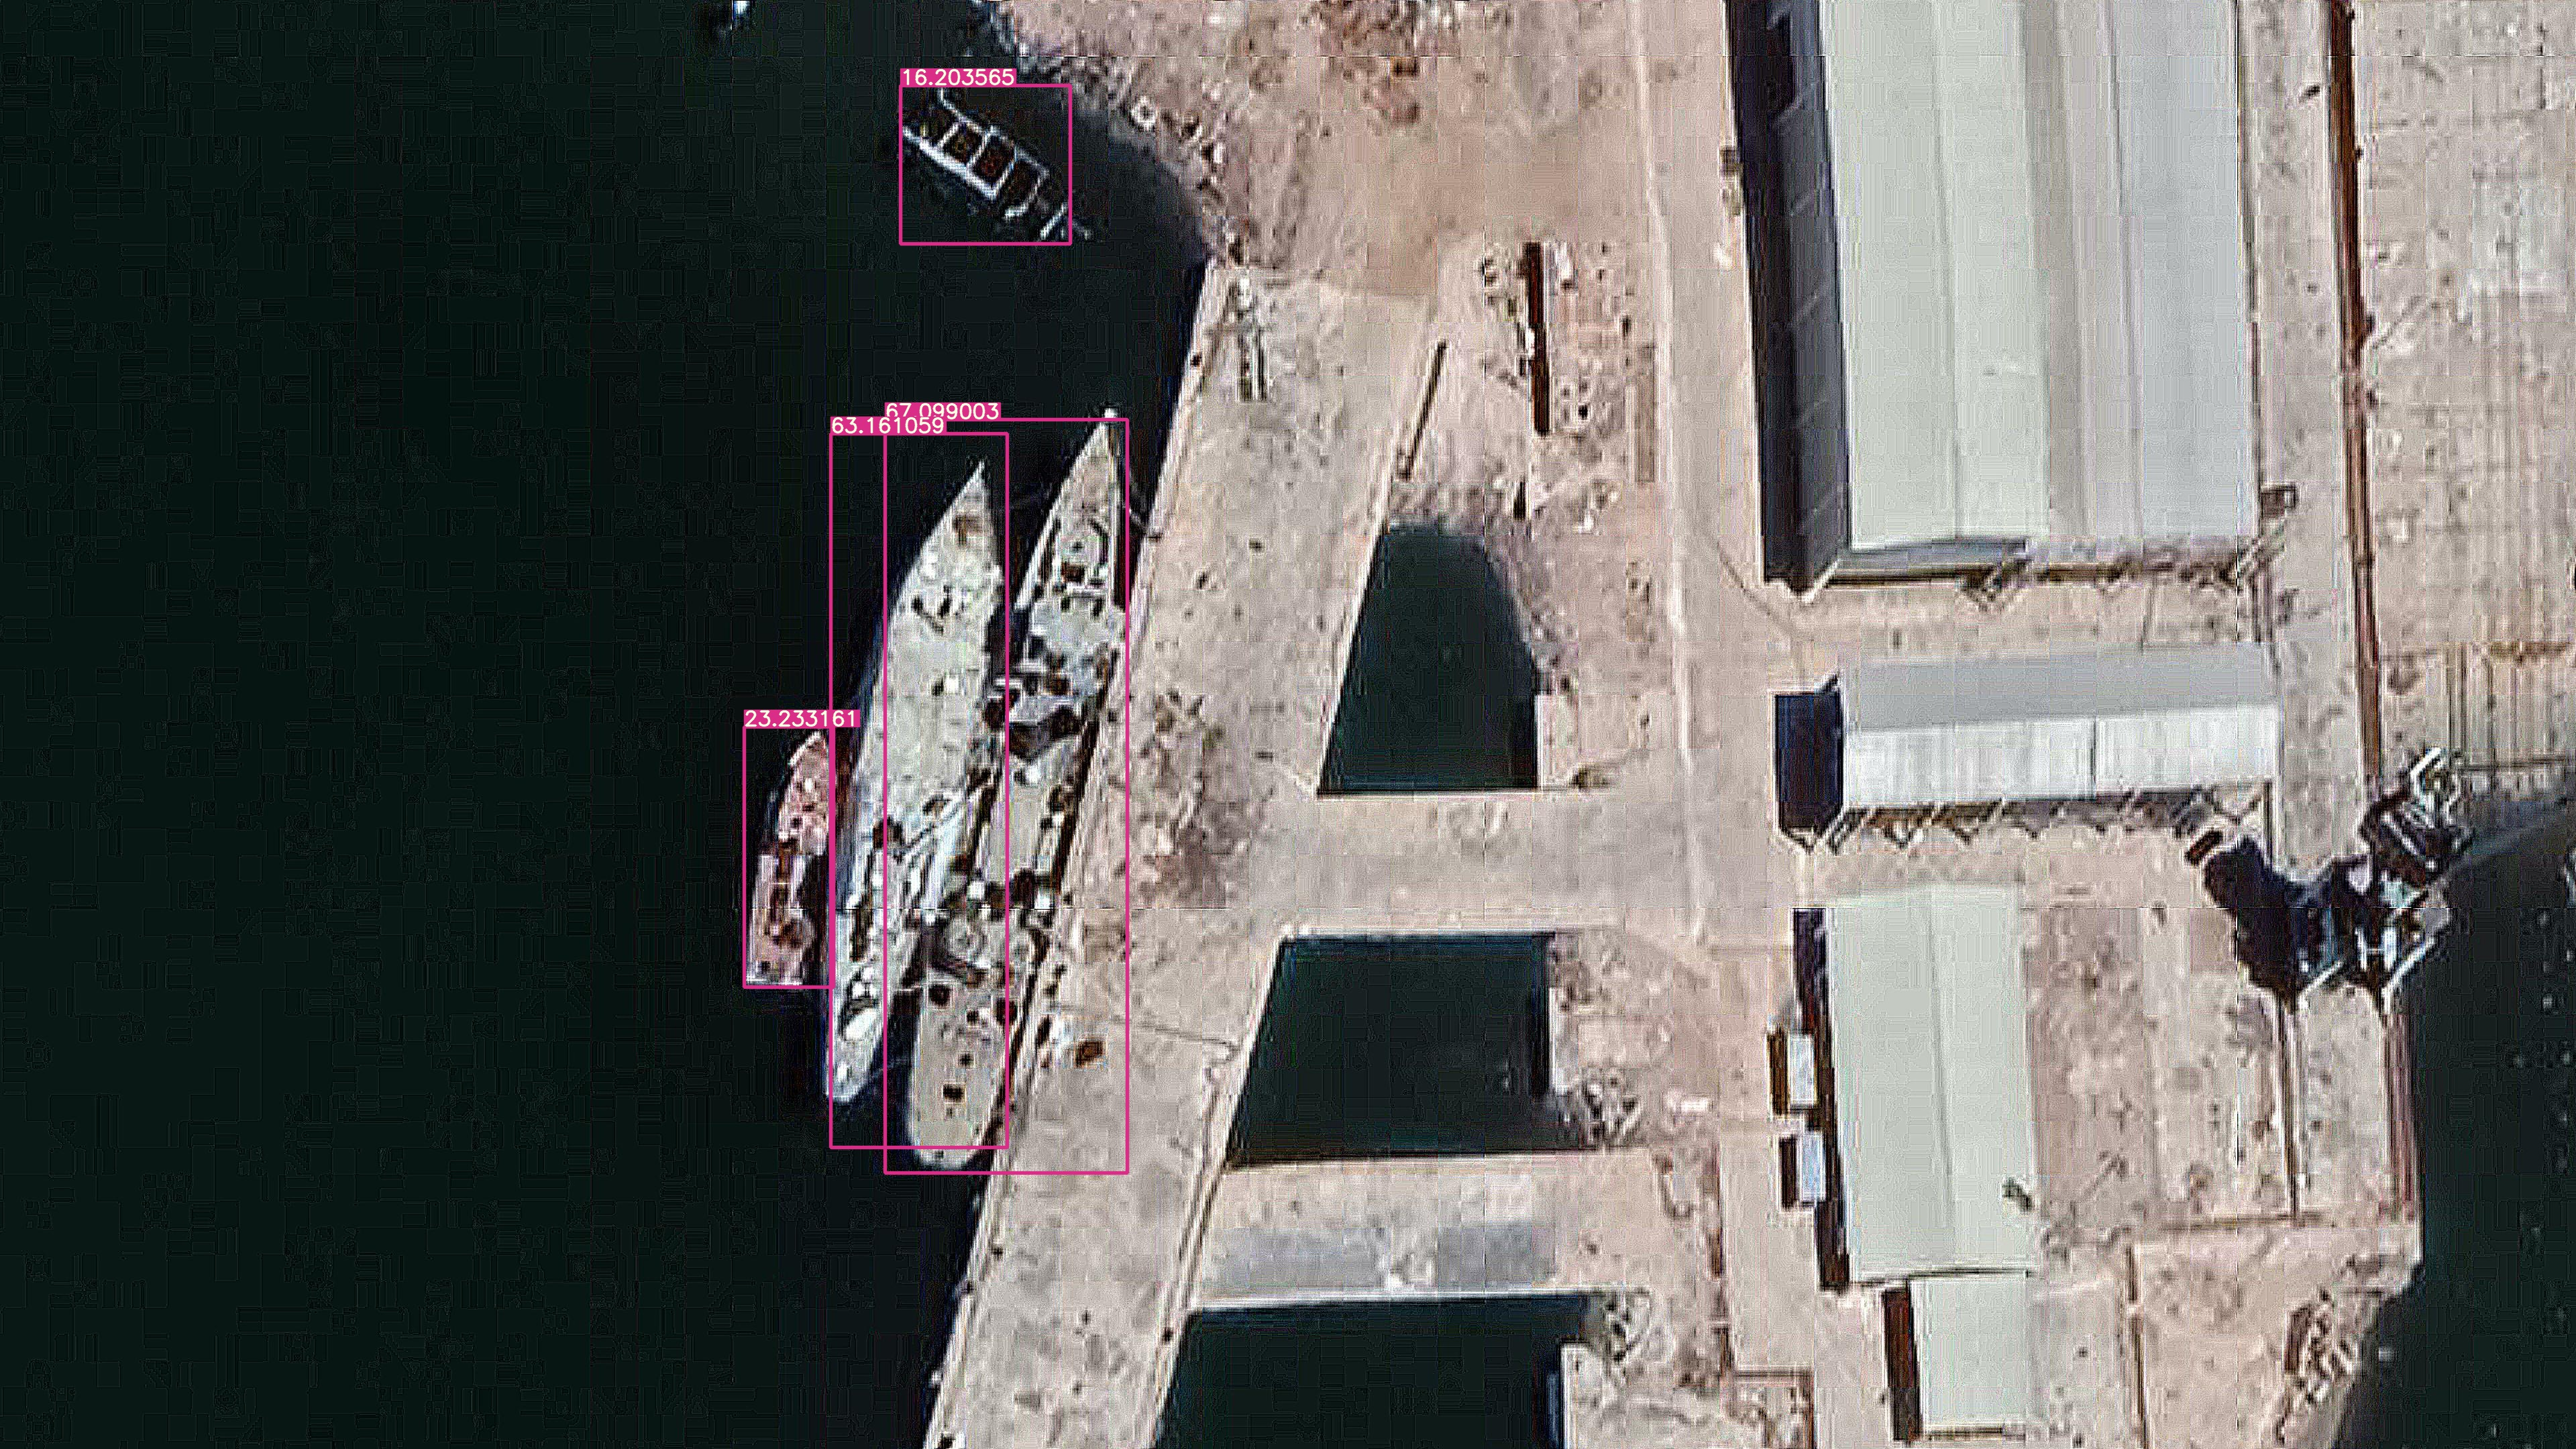
\includegraphics[scale=0.11]{img/Guaymas_202105_detect_small_large.jpg}
    \caption{The algorithm can detect all the boats (May 2021, Guaymas) well if no big boats overflowed the image.}
    \label{fig:Guaymas_202105_detect_small_large}
\end{figure}




\subsection{Classification of Entertainment Boats and Fishing Boats}
\label{sec:3.2.5}
After distinguishing between large and small boats, it is necessary to distinguish between small recreational boats for domestic use and fishing boats without a roof. In this thesis, whether or not the colour shown on satellite images of detected small boats is mostly white becomes a feature that distinguishes recreational boats from fishing boats. To do this, we need to find the range of small boats previously identified by the algorithm, i.e. the four coordinates of the anchor box. Then, analyse whether the colour within the anchor frame is white or close to white. Finally, the number of white boats is counted.


\section{Workflow}
The flow chart from the training data to the final statistics made is shown in Figure~\ref{fig:workflow}.
\begin{figure}[h]
    \centering
    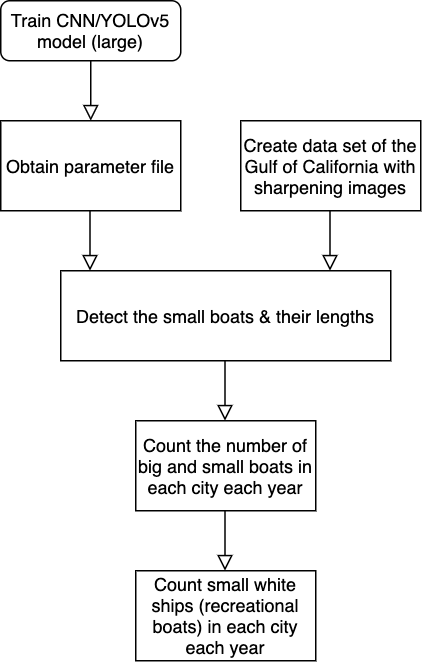
\includegraphics[scale=0.6]{img/workflow.png}
    \caption{The workflow of detection.}
    \label{fig:workflow}
\end{figure}